\chapter{Background Research: Recommender Systems}

This section introduces the fundamental concepts of recommender and machine learning systems. Then, it discusses different use cases as well as techniques. Finally, it illustrates some of the algorithms recommender systems rely on.

\section{Definition}

Recommendations are neither a new idea nor limited to the digital age. \citet{ricci11} write that traditional recommendations can be observed in various scenarios, such as a peer's recommendation when buying a book or reviews when choosing a movie. The authority of the recommender has an important role in the acceptance of the recommendation. A renowned film critic may appear more credible than a random colleague. When it comes to car parts, a mechanist may be a good candidate to ask. However the authority is not only limited to expertise -- in fact we tend to rely more on recommendations which put our personal experiences and preferences into account. A previous companion for a wonderful trip can certainly have a better authority than a travel agent.

As mentioned in the introduction, with the growth of the Internet, the amount of information available on the Web increased rapidly. Especially major e-commerce Web sites were extending their range of products and services. Although a wider and varied range of items is initially good for the user, users found it more and more difficult to find the appropriate items or make the right choices. Web sites have deployed different type of solutions -- such as search engines and more user friendly interfaces -- to cope with this problem.

Another approach are recommender systems which basically provides a bespoke collection of items with the intention to highlight relevant items to a user. Depending on the recommending technique various data sources are taken into account being the user's context or previous interactions. It is a continuous learning process. The more it learns, the more accurate the recommendations will become. The user's behaviour on given recommendations are further a powerful learning source for the system -- e.g. if the user tends to accept some recommendations over others -- to tweak the recommendations. Most recommender systems concentrate on guiding the user towards new, unexperienced items \cite{ricci11}.

Recommender systems are autonomous and utilize machine learning principles which is a branch of artificial intelligence (AI). Latter is defined by \citet{mccarthy07} as \textit{'the science and engineering of making intelligent machines, especially intelligent computer programs'}. In that sense, machine learning enables computers to learn from data passed through it to be able to make predictions about future data. In other words the learning machine tries to generalize. It is based on the assumption that almost all data includes \textit{patterns} -- any repeating regularity that describes the \textit{model} the learning machine is concerned about. This allows learning machines to generalise \cite{segaran07}.\label{bg-def-machinelearning}



\section{Adoption}

\citet{ricci11} note that research on recommender systems is relatively new compared to other classical information retrieval methods like databases and search engines. However it is gaining attention due to various reasons. First of all e-commerce companies including Amazon, YouTube and Netflix invest a lot in recommender systems. As trendsetters and pioneers for other institutions they build a demand for further research and development. Dedicated conferences and academic courses as well as its adaption in several academic journals are indicators of recognition of this research area.

E-commerce companies running recommender systems hope among others to increase number of items sold, sell more diverse items, increase customer satisfaction and recommend sequences plus bundles \cite{ricci11}. I will illustrate the usage with two examples.

\subsection{Netflix}

\begin{figure}[ht]
    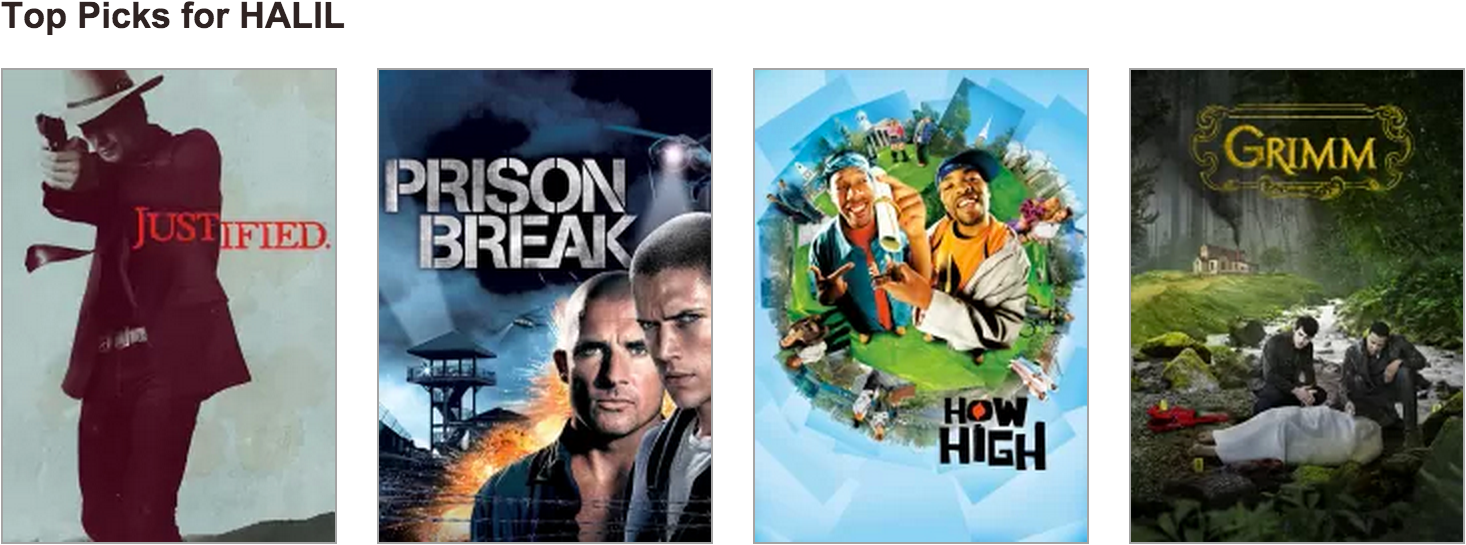
\includegraphics[width=\textwidth,center]{background/adoption/netflix.png}
    \caption{Netflix Recommendations}
    \label{fig:netflix}
\end{figure}

Netflix offers their on-demand video streaming with a simplified user interface across all platforms including smartphones and tablets. There is only limited functionality to navigate through their items. It rather focuses on ranked lists around a topic or genre. Once subscribers start using their service, the recommender system of Netflix on one hand builds new, personalised lists in relation to that item. On the other hand it updates existing lists with that learning.

Their recommender system is such a fundamental part of their business model that they launched a competition called Netflix Prize and called expert teams to propose a more accurate algorithm. They eventually awarded a million dollar to best scoring team \cite{netflix09}.

\subsection{Amazon}
\label{bg-adopt-amazon}

\begin{figure}[ht]
    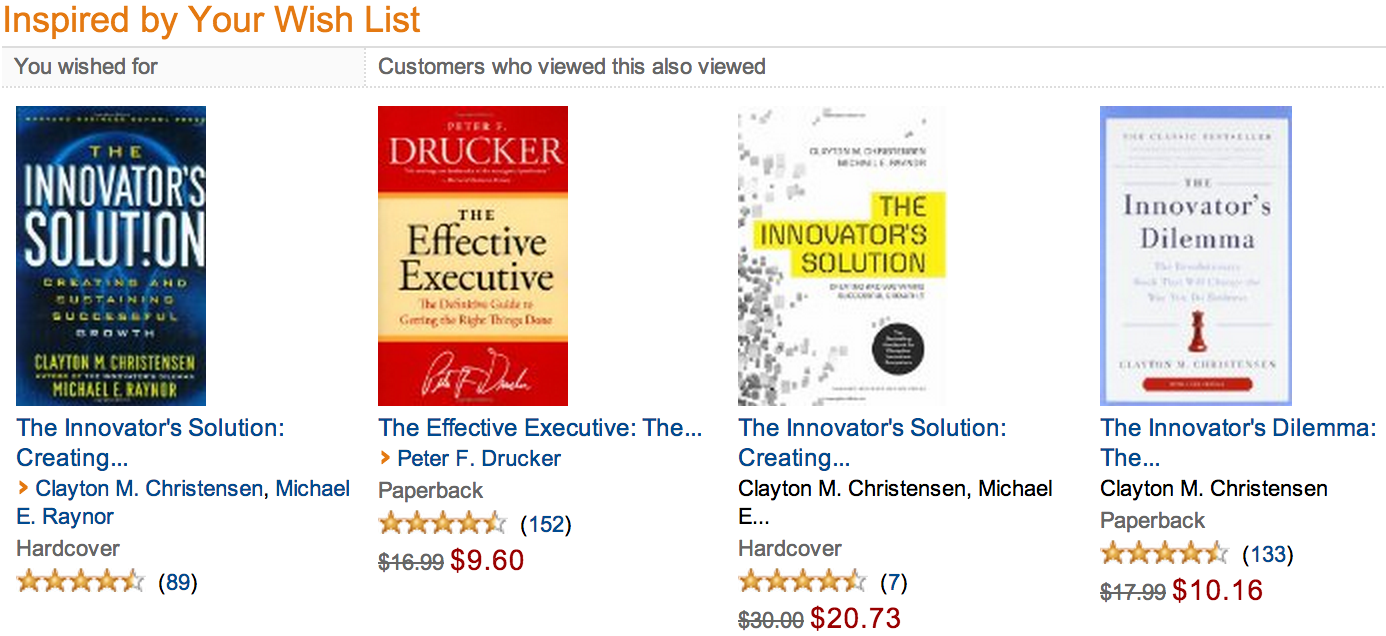
\includegraphics[width=\textwidth,center]{background/techniques/amazon.png}
    \caption{Item-to-Item Recommendations by Amazon}
    \label{fig:itembased-amazon}
\end{figure}

The online retailer Amazon relies on recommender systems throughout their e-commerce platform. They are not limited to the website but are in fact also used in their email campaigns. Amazon inventend \textit{item-based collaborative filtering} which surprisingly focuses on items rather than users and is discussed in detail in section \ref{bg-tech-itembased} \cite{linden03}. The user's collaboration is taken into account to put items into relation.

Moreover Amazon is an examplary user of \textit{automated merchandising} to which I could not find any coverage in literature, although it is an important area for e-commerce companies. Recommender systems are observing the behaviour of the customer on the item collection to predict individual recommendations. However this behaviour can also be used to build objective relations between items such as categorisation and cross-selling (offer additional items to increase basket value). Given that Amazon has more than 200 million products at the time of writing, merchandising the whole catalog manually is almost impossible.



\section{Techniques}

In the course of development different techniques to building recommendations emerged. Fundamentally techniques are classified by the information sources they use. The sources of personalised recommendations are typically user-item interactions (\textit{collaborative filtering}), item features (\textit{content-based filtering}), user features (\textit{demographic filtering}) as well as knowledge about the user and item (\textit{knowledge-based filtering}). Non-personalised recommendations also exist in form of ranked lists such as top sellers or related items. However they are typically not part of the research in recommender systems.

\citet{anand03} differentiate between \textit{explicit} and \textit{implicit} data collection. Information the user intentionally provides to the system to express a positive preference to items are referred to as \textit{explicit} data collection including rating an item, adding it to a wish list or liking it. \textit{Implicit} data on the other hand is collected by observing the user's behaviour e.g. usage of navigation and search elements or purchase of items.

\subsection{Collaborative Filtering}
\label{bg-tech-collaborative}

\begin{figure}[ht]
    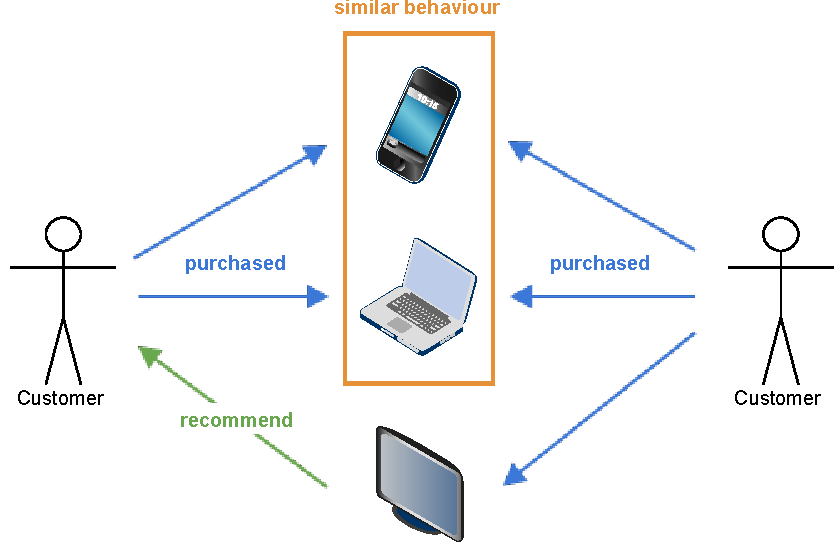
\includegraphics[width=\textwidth,center]{background/techniques/collaborative.pdf}
    \caption{Collaborative Filtering}
    \label{fig:collaborative}
\end{figure}

Basically this technique recommends items other users with similar preferences interacted with e.g. liked or purchased. In order to do this the recommender system needs to observe users' behaviours and interactions. Based on these learnings, it will then look up other users with similar behaviour patterns and build recommendations from their preferences -- preferrably items which the original user has not experienced yet (see figure \ref{fig:collaborative}).

The major advantage of the collaborative filtering approach is that the recommender system does not require any knowledge about the items.

\subsubsection{Item-to-Item Collaborative Filtering}
\label{bg-tech-itembased}

\begin{figure}[ht]
    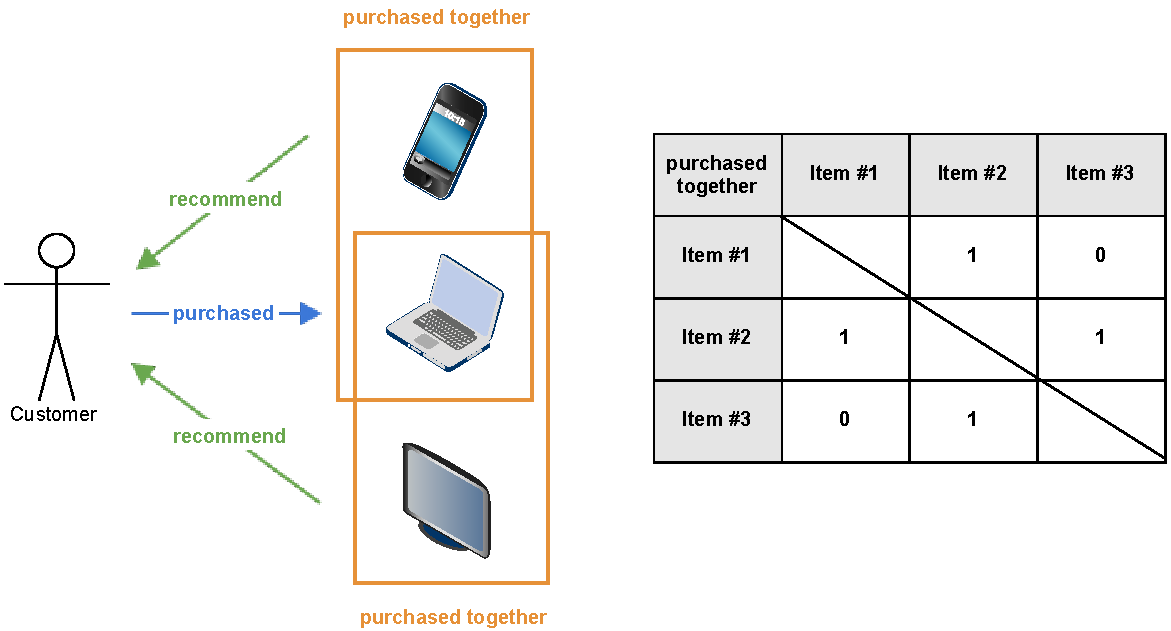
\includegraphics[width=\textwidth,center]{background/techniques/itembased.pdf}
    \caption{Item-to-Item Collaborative Filtering}
    \label{fig:itembased}
\end{figure}

This approach is a derivative of traditional collaborative filtering methods and has been popularised by Amazon (see figure \ref{fig:itembased-amazon}). The fundamental difference lies in the fact that the item-to-item approach collects collaborative data to put items into relation with other items rather than users. Figure \ref{fig:itembased} shows an example of items purchased together. The recommendation query takes an item -- currently viewed or from a wish list -- as an argument and looks for items purchased together with that item.

Given that the item range can be very wide, item-to-item filtering methods require significant computing time and data storage. However they are usually preprocessed offline thus queries can be processed rather quickly.

\subsection{Content-Based Filtering}

\begin{figure}[ht]
    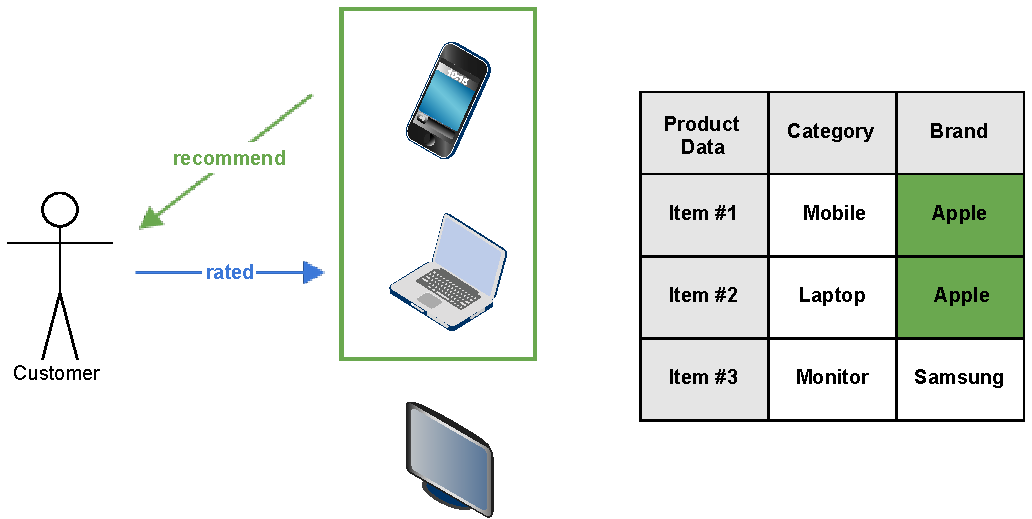
\includegraphics[width=\textwidth,center]{background/techniques/contentbased.pdf}
    \caption{Content-Based Filtering}
    \label{fig:contentbased}
\end{figure}

Content-based recommendation methods make use of item features to find similar items. Based on items the user has showed a positive preference to before -- such as rated or purchased -- other similar items are looked up based on the item's features. Figure \ref{fig:contentbased} illustrates a customer who has rated an item positively. The recommender system compares the rated item with other items, finds another item which has the same brand and therefore recommends that item.

\subsection{Demographic Filtering}

The demographic filtering is similar to the content-based method with the significant difference that demographic filtering examines the demographic profile of a user -- user features rather than item features -- to find similar users and recommend items those users have showed positive preference to in the past. \citet{ricci11} makes the assumption that recommendations should be different for demographic groups. The demographic profile can consist of age, gender, interests, language, country etc. To give an example, a hotel search engine may want to recommend different hotels to a business person and different ones for a young couple.

\subsection{Knowledge-Based Filtering}

Recommendations of knowledge-based systems rely on specific domain -- often manual -- knowledge about how useful items are for a user \cite{ricci11}. These systems are usually constraint-based or case-based. Both approaches are similar in their conversational process. In other words, the user specifies the requirements and the system tries to find solutions which are fulfilling them. Whereas constraint-based systems are matching the requirements explicitly (such as price ranges), case-based systems make us of similarity measures (e.g. distance to a point of interest).

\subsection{Hybrids}

Hybrid recommender systems combine the beforementioned techniques. One possible motivation of using hybrid systems may be to overcome weaknesses of one approach by combining it with another. However there are many possible ways of combining techniques. \citet{burke07} identified seven different types:

\begin{description}
    \item[Weighted] The scores of recommender components are combined numerically.
    \item[Switching] The system chooses one over other components.
    \item[Mixed] Recommendations from components are presented together.
    \item[Feature Combination] Features from different sources are combined and passed to a single component.
    \item[Feature Augmentation] One component augments the knowledge source, which is then the input of the next component.
    \item[Cascade] Components are given strict priorities with the lower prioritised ones breaking ties of the higher ones.
    \item[Meta-Level] Similar to \textit{feature agumentation} yet first component completely replaces -- instead of augments -- the initial source.
\end{description}



\section{Algorithms}

As discussed in section \ref{bg-def-machinelearning} recommender systems rely heavily on machine learning practices. In that sense it is not surprising that most algorithms recommender systems use are derived from that discipline. Algorithms are usually defined to solve a specific problem and it is therefore crucial to utilise the right algorithm to get the expected results.

In the next two sections I will illustrate two algorithms which are very popular in recommender systems.

\subsection{Pearson Correlation Coefficient}

\begin{figure}[ht]
    \[Pearson_(A,B) = \frac{\sum ab - \frac{\sum a \sum b}{N}}{\sqrt{(\sum a^{2} - \frac{(\sum a)^{2}}{N})(\sum b^{2} - \frac{(\sum b)^{2}}{N})}}\]
    \caption{Pearson Correlation Coefficient}
    \label{fig:pearson}
\end{figure}

The \textit{Pearson correlation coefficient} provides a measure to calculate the correlation of two variables. In the recommender systems context it is useful to compare user's behaviour patterns or preferences \cite{segaran07}. The coefficient is defined to be between 1 to -1 where 1 indicates a perfect correlation, 0 no correlation and -1 a perfectly inverse correlation.

\subsection{Tanimoto Coefficient}

\begin{figure}[ht]
    \[T = \frac{N_{ab}}{(N_a + N_b - N_{ab})}\]
    \caption[Tanimoto coefficient]{Tanimoto coefficient where \(N_a\) respectively \(N_b\) is the count of properties of \(a\) respectively \(b\) and \(N_{ab}\) is the count of intersecting properties.}
    \label{fig:tanimoto}
\end{figure}

The \textit{Tanimoto coefficient} tells us the similarity of two sets \cite{segaran07}. It can be used to measure how similar two items or users are based on their features which is useful for \textit{content-based} and \textit{demographic filtering} methods. Below is an example of two items which we want to compare:

\lstset{language=Python}
\begin{lstlisting}
    A = [mobile, apple, iphone, black, 32G]
    B = [mobile, apple, ipad, black]
\end{lstlisting}

Given the equation in figure \ref{fig:tanimoto} we come to the conclusion: \[T = \frac{N_{ab}}{(N_a + N_b - N_{ab})} = \frac{3}{5 + 4 - 3} = 0.5\]